%!TEX root = dolgozat.tex
%%%%%%%%%%%%%%%%%%%%%%%%%%%%%%%%%%%%%%%%%%%%%%%%%%%%%%%%%%%%%%%%%%%%%%%
\chapter{Results and evaluation}\label{ch:elemzes}

\section{Metrics}

\subsection{Encryption/decryption speed}

Since the major features of the application revolve around data security and encryption,
it is important to select the correct methodology for data protection in terms of both efficiency and security \cite{singh2013study}.
\emph{AES-256} is a flexible, yet extremely secure option in terms of information protection.
Although it is virtually impenetrable using brute-force methods, in terms of resources it is less efficient than the \emph{DES (data encryption standard) algorithms}.

\begin{figure}[H]
	\centering
	\definecolor{mycolor1}{rgb}{0.00000,0.44700,0.74100}%
\definecolor{mycolor2}{rgb}{0.85000,0.32500,0.09800}%
\definecolor{mycolor3}{rgb}{0.92900,0.69400,0.12500}%
%
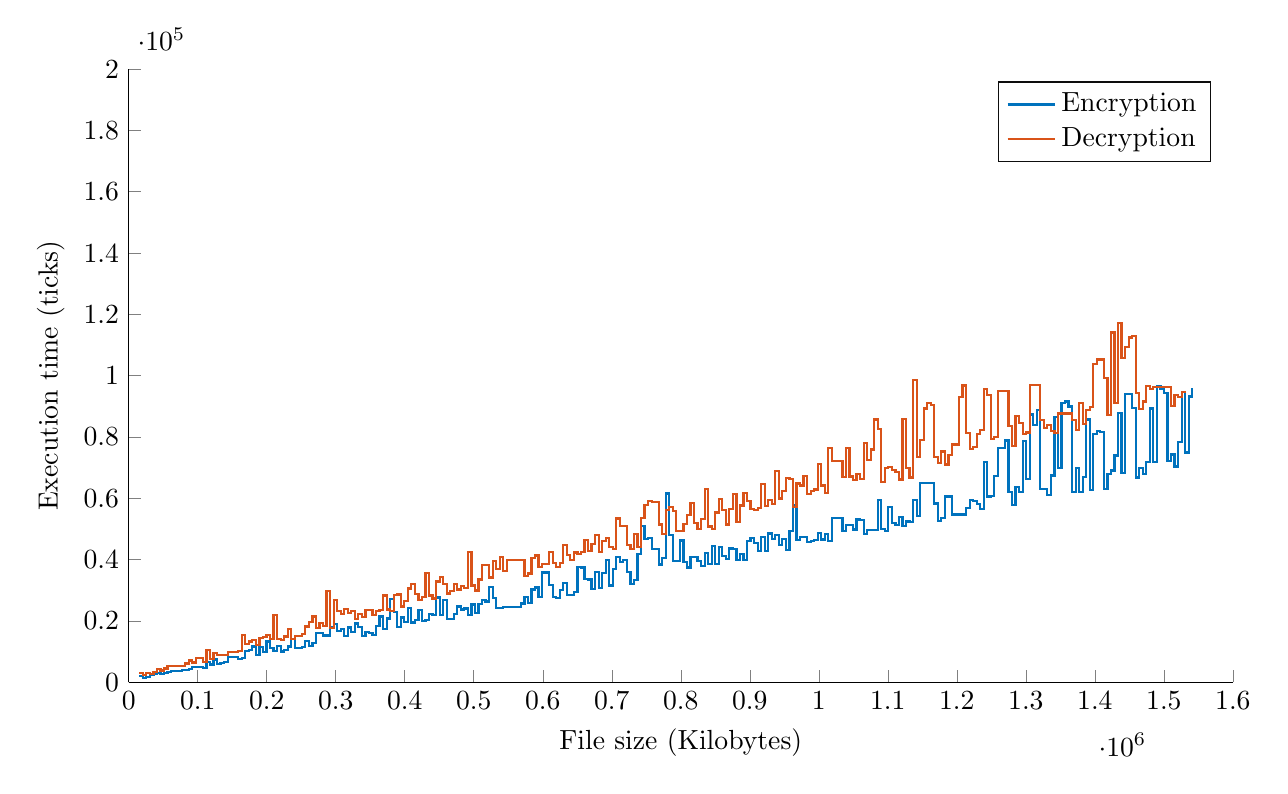
\begin{tikzpicture}

\begin{axis}[%
width=5.520833in,
height=3.065625in,
at={(1in,2in)},
scale only axis,
xmin=0,
xmax=1600000,
xlabel={File size (Kilobytes)},
ymin=0,
ymax=200000,
ylabel={Execution time (ticks)},
axis x line*=bottom,
axis y line*=left,
legend style={legend cell align=left,align=left,draw=white!5!black}
]
\addplot[const plot,color=mycolor1,line width=0.8pt,mark size=1.0pt,mark=.,mark options={solid}] plot table[row sep=crcr] {%
15360 2018 \\
20480 1357 \\
25600 1591 \\
30720 2498 \\
35840 2639 \\
40960 3029 \\
46080 2787 \\
51200 3145 \\
56320 3472 \\
61440 3755 \\
66560 3638 \\
71680 3564 \\
76800 4115 \\
87040 4307 \\
92160 4963 \\
102400 4870 \\
107520 4779 \\
112640 6593 \\
117760 5766 \\
122880 7444 \\
128000 5969 \\
133120 6374 \\
138240 6624 \\
143360 8358 \\
148480 8198 \\
158720 7587 \\
163840 7985 \\
168960 10085 \\
174080 10472 \\
179200 11641 \\
184320 8960 \\
189440 11437 \\
194560 9957 \\
199680 13331 \\
204800 11080 \\
209920 10291 \\
215040 11825 \\
220160 10043 \\
225280 10438 \\
230400 11665 \\
235520 14040 \\
240640 11276 \\
245760 11293 \\
250880 11471 \\
256000 13528 \\
261120 11847 \\
266240 12915 \\
271360 16094 \\
276480 16106 \\
281600 15251 \\
291840 17883 \\
296960 18958 \\
302080 16604 \\
307200 17276 \\
312320 15151 \\
317440 17860 \\
322560 16281 \\
327680 19143 \\
332800 18058 \\
337920 15081 \\
343040 16324 \\
348160 16002 \\
353280 15300 \\
358400 18342 \\
363520 21446 \\
368640 17409 \\
373760 20767 \\
378880 27074 \\
384000 22992 \\
389120 18067 \\
394240 21159 \\
399360 19668 \\
404480 24201 \\
409600 19469 \\
414720 20307 \\
419840 23584 \\
424960 19998 \\
430080 20433 \\
435200 22381 \\
440320 22013 \\
445440 27650 \\
450560 22065 \\
455680 26858 \\
460800 20586 \\
465920 20583 \\
471040 22196 \\
476160 24696 \\
481280 23727 \\
486400 24082 \\
491520 21874 \\
496640 25353 \\
501760 22471 \\
506880 25445 \\
512000 26921 \\
517120 26333 \\
522240 30998 \\
527360 27583 \\
532480 24332 \\
537600 24176 \\
542720 24503 \\
568320 25723 \\
573440 27844 \\
578560 25805 \\
583680 30270 \\
588800 30891 \\
593920 27697 \\
599040 35783 \\
609280 31749 \\
614400 27735 \\
619520 27468 \\
624640 30130 \\
629760 32453 \\
634880 28522 \\
645120 29331 \\
650240 37720 \\
655360 37408 \\
660480 33583 \\
665600 33526 \\
670720 30320 \\
675840 35929 \\
680960 30644 \\
686080 35664 \\
691200 39906 \\
696320 31537 \\
701440 36834 \\
706560 40858 \\
711680 39346 \\
716800 39904 \\
721920 35975 \\
727040 31927 \\
732160 33434 \\
737280 41742 \\
742400 50994 \\
747520 46849 \\
752640 46972 \\
757760 43353 \\
768000 38407 \\
773120 40474 \\
778240 61574 \\
783360 48102 \\
788480 39538 \\
793600 39543 \\
798720 46258 \\
803840 39234 \\
808960 37406 \\
814080 40960 \\
819200 40752 \\
824320 39588 \\
829440 37850 \\
834560 42111 \\
839680 38641 \\
844800 44358 \\
849920 38521 \\
855040 44214 \\
860160 41120 \\
865280 40333 \\
870400 43604 \\
875520 43414 \\
880640 39986 \\
885760 41903 \\
890880 39896 \\
896000 46141 \\
901120 47058 \\
906240 45466 \\
911360 42942 \\
916480 47424 \\
921600 42783 \\
926720 48551 \\
931840 46662 \\
936960 48113 \\
942080 44889 \\
947200 46631 \\
952320 43063 \\
957440 49236 \\
962560 57885 \\
967680 46493 \\
972800 47425 \\
977920 47431 \\
983040 45642 \\
988160 45991 \\
993280 46480 \\
998400 48660 \\
1003520 46578 \\
1008640 48315 \\
1013760 46113 \\
1018880 53515 \\
1034240 49470 \\
1039360 51201 \\
1044480 51270 \\
1049600 49855 \\
1054720 53067 \\
1059840 52876 \\
1064960 48322 \\
1070080 49762 \\
1085440 59417 \\
1090560 50088 \\
1095680 49403 \\
1100800 57204 \\
1105920 51849 \\
1111040 51313 \\
1116160 53839 \\
1121280 50976 \\
1126400 52408 \\
1131520 52156 \\
1136640 59547 \\
1141760 54125 \\
1146880 64925 \\
1167360 58298 \\
1172480 52506 \\
1177600 53479 \\
1182720 60605 \\
1192960 54752 \\
1213440 56962 \\
1218560 59471 \\
1223680 59170 \\
1228800 58236 \\
1233920 56605 \\
1239040 71838 \\
1244160 60592 \\
1249280 60771 \\
1254400 67252 \\
1259520 76426 \\
1264640 76324 \\
1269760 78831 \\
1274880 62016 \\
1280000 57834 \\
1285120 63712 \\
1290240 61992 \\
1295360 78662 \\
1300480 66388 \\
1305600 87359 \\
1310720 83936 \\
1315840 88816 \\
1320960 63116 \\
1326080 63032 \\
1331200 61154 \\
1336320 67428 \\
1341440 86638 \\
1346560 69867 \\
1351680 91105 \\
1356800 91611 \\
1361920 89949 \\
1367040 62075 \\
1372160 69961 \\
1377280 61957 \\
1382400 66898 \\
1387520 85745 \\
1392640 62746 \\
1397760 80879 \\
1402880 81967 \\
1408000 81637 \\
1413120 63158 \\
1418240 67912 \\
1423360 69089 \\
1428480 73945 \\
1433600 87884 \\
1438720 68270 \\
1443840 94084 \\
1448960 93958 \\
1454080 89500 \\
1459200 66778 \\
1464320 69808 \\
1469440 67965 \\
1474560 71877 \\
1479680 89308 \\
1484800 71806 \\
1489920 96449 \\
1495040 95678 \\
1500160 94474 \\
1505280 72222 \\
1510400 74279 \\
1515520 70375 \\
1520640 78419 \\
1525760 94683 \\
1530880 74933 \\
1536000 93221 \\
1541120 95945 \\
};
\addlegendentry{Encryption};

\addplot[const plot,color=mycolor2,line width=0.8pt,mark size=1.0pt,mark=.,mark options={solid}] plot table[row sep=crcr] {%
15360 3068 \\
20480 2364 \\
25600 2902 \\
30720 2775 \\
35840 3245 \\
40960 4389 \\
46080 3856 \\
51200 4475 \\
56320 5258 \\
61440 5252 \\
71680 5429 \\
76800 5206 \\
81920 6130 \\
87040 7085 \\
92160 6458 \\
97280 7929 \\
107520 6714 \\
112640 10491 \\
117760 7716 \\
122880 9526 \\
128000 8803 \\
133120 8981 \\
138240 8815 \\
143360 9982 \\
148480 9949 \\
158720 10162 \\
163840 15312 \\
168960 12418 \\
174080 13302 \\
179200 13815 \\
184320 12227 \\
189440 14479 \\
194560 14772 \\
199680 15387 \\
204800 14207 \\
209920 21999 \\
215040 14018 \\
220160 13883 \\
225280 14950 \\
230400 17365 \\
235520 14132 \\
240640 14975 \\
245760 15144 \\
250880 15739 \\
256000 18159 \\
261120 19694 \\
266240 21478 \\
271360 17662 \\
276480 19315 \\
281600 18429 \\
286720 29777 \\
291840 17618 \\
296960 26890 \\
302080 23268 \\
307200 22142 \\
312320 23991 \\
317440 22699 \\
322560 23238 \\
327680 20657 \\
332800 22368 \\
337920 21347 \\
343040 23482 \\
348160 23502 \\
353280 21899 \\
358400 23296 \\
363520 23508 \\
368640 28314 \\
373760 23730 \\
378880 23163 \\
384000 28347 \\
389120 28598 \\
394240 24683 \\
399360 26383 \\
404480 30613 \\
409600 32140 \\
414720 28858 \\
419840 26843 \\
424960 27782 \\
430080 35721 \\
435200 28329 \\
440320 27330 \\
445440 32880 \\
450560 34461 \\
455680 32056 \\
460800 28949 \\
465920 29774 \\
471040 31987 \\
476160 30263 \\
481280 31425 \\
486400 30659 \\
491520 42405 \\
496640 31554 \\
501760 29907 \\
506880 33554 \\
512000 38345 \\
522240 34166 \\
527360 39612 \\
532480 36935 \\
537600 40919 \\
542720 36329 \\
547840 39955 \\
573440 34750 \\
578560 35503 \\
583680 40421 \\
588800 41380 \\
593920 37596 \\
599040 38545 \\
609280 42491 \\
614400 38796 \\
619520 37593 \\
624640 38921 \\
629760 44826 \\
634880 41472 \\
640000 39994 \\
645120 42347 \\
650240 41878 \\
655360 42548 \\
660480 46473 \\
665600 42915 \\
670720 45103 \\
675840 48051 \\
680960 42493 \\
686080 46169 \\
691200 47090 \\
696320 44076 \\
701440 43483 \\
706560 53429 \\
711680 51044 \\
721920 44768 \\
727040 43595 \\
732160 48413 \\
737280 44104 \\
742400 53609 \\
747520 57877 \\
752640 59118 \\
757760 58808 \\
768000 51460 \\
773120 48340 \\
778240 56085 \\
783360 57179 \\
788480 55971 \\
793600 49282 \\
803840 51573 \\
808960 54472 \\
814080 58405 \\
819200 51957 \\
824320 50115 \\
829440 53235 \\
834560 63102 \\
839680 50800 \\
844800 49872 \\
849920 55402 \\
855040 59735 \\
860160 56138 \\
865280 51480 \\
870400 56493 \\
875520 61505 \\
880640 52364 \\
885760 57642 \\
890880 61837 \\
896000 59193 \\
901120 56479 \\
906240 56117 \\
911360 56929 \\
916480 64725 \\
921600 57452 \\
926720 59476 \\
931840 58158 \\
936960 68887 \\
942080 59955 \\
947200 62406 \\
952320 66730 \\
957440 66414 \\
962560 57054 \\
967680 64871 \\
972800 64207 \\
977920 67162 \\
983040 61336 \\
988160 62373 \\
993280 62882 \\
998400 71250 \\
1003520 64169 \\
1008640 61717 \\
1013760 76290 \\
1018880 72096 \\
1034240 67002 \\
1039360 76511 \\
1044480 67124 \\
1049600 65937 \\
1054720 67993 \\
1059840 66257 \\
1064960 77925 \\
1070080 72437 \\
1075200 75919 \\
1080320 85705 \\
1085440 82641 \\
1090560 65301 \\
1095680 69996 \\
1100800 70172 \\
1105920 69133 \\
1111040 68685 \\
1116160 66118 \\
1121280 85934 \\
1126400 69846 \\
1131520 66778 \\
1136640 98608 \\
1141760 73523 \\
1146880 79052 \\
1152000 89318 \\
1157120 91090 \\
1162240 90516 \\
1167360 73422 \\
1172480 71586 \\
1177600 75257 \\
1182720 71008 \\
1187840 74084 \\
1192960 77559 \\
1203200 93028 \\
1208320 96833 \\
1213440 81241 \\
1218560 75969 \\
1223680 76858 \\
1228800 80982 \\
1233920 82308 \\
1239040 95678 \\
1244160 93605 \\
1249280 79229 \\
1254400 80130 \\
1259520 94947 \\
1264640 95030 \\
1274880 83502 \\
1280000 77134 \\
1285120 86858 \\
1290240 84628 \\
1295360 80924 \\
1300480 81470 \\
1305600 97093 \\
1320960 85634 \\
1326080 83026 \\
1331200 84031 \\
1336320 82088 \\
1341440 81379 \\
1346560 87653 \\
1367040 85559 \\
1372160 82211 \\
1377280 90993 \\
1382400 84255 \\
1387520 88830 \\
1392640 89810 \\
1397760 103863 \\
1402880 105300 \\
1413120 99202 \\
1418240 87192 \\
1423360 114108 \\
1428480 90977 \\
1433600 117293 \\
1438720 105769 \\
1443840 109451 \\
1448960 112478 \\
1454080 112945 \\
1459200 94379 \\
1464320 89150 \\
1469440 91580 \\
1474560 96677 \\
1479680 95600 \\
1484800 96290 \\
1510400 90062 \\
1515520 93667 \\
1520640 93016 \\
1525760 94605 \\
1530880 94974 \\
};
\addlegendentry{Decryption};

\end{axis}
\end{tikzpicture}

	\caption{Encryption/Decryption duration over file size}
\end{figure}

As the above graph illustrates, the cryptographic operations have a linear (O(n)) time complexity, the decryption being slightly more demanding in general.
In real-life scenarios the majority of the documents handled by the application do not reach 10 MB in size.
This denotes that generally the cryptographic operations for a single document would not cross 15 milliseconds.
\emph{Note: the measurements were taken using an Intel\textregistered  Core\texttrademark  i7-4790K CPU @ 4.00 GHz processor and 16 GB of DDR3 RAM on a desktop PC.}

\section{System requirements}

From a hardware point of view, the application falls into the ligh-weight category, since it is not using algorithms with high time- or space-complexity.
A major factor regarding the physical capabilities of the server is the size of the userbase, the scale of the application.
Although the server can run on machines with fairly low performance with ease, a high number of consecutive requests can drastically influence 
performance or even cause server outage or failure.
Taking this into consideration, the recommended specifications are estimated to be capable of handling approximately \emph{10 000 users}.

\subsection{Recommended hardware specifications}

\subsubsection{Web Server (\emph{including database server})} 

\begin{itemize}
	\item CPU: Octa-Core 2.8 GHz CPU or higher
	\item RAM: 16 GB available RAM (DDR4) or higher
	\item Storage: 50 GB available hard disk space
\end{itemize}

\subsubsection{Mobile application}

\begin{itemize}
	\item CPU: Qualcomm\textregistered Snapdragon\texttrademark 765 or newer
	\item RAM: 2 GB available RAM
	\item Storage: 4 GB of non-volatile storage
	\item Rear camera: 720p resolution or higher
\end{itemize}

\subsection{Software requirements}

\subsubsection{Web Server}

\begin{itemize}
	\item Microsoft Windows Server 2012 or 2012 R2 operating system
	\item .NET 5 runtime + Hosting Bundle for IIS Support
	\item IIS 10.0
	\item Microsoft OLE DB Driver 18 for SQL Server
	\item Microsoft SQL Server 2019
	\item Microsoft SQL Server Management Studio (or optionally HeidiSQL)
\end{itemize}

\subsubsection{Mobile application}

\begin{itemize}
	\item Android 10.0 (Q)
\end{itemize}

\section{Obstacles and difficulties}

As expected, no application development process exists without its intricacies and E-me is no exception.
In the course of one year, there were multiple obstacles and difficulties that had to be tackled in order to create the current version of the application,
some of them slowing down the development process by days or even weeks.

These impediments provided a great deal of knowledge when it comes to preemtive thinking and the organization of a work process that requires multiple
steps and layers to complete.
In my opinion, the majority of the following obstacles are easily avoidable with in-depth analysis of the technologies and processes that build up the application.

\subsection{HTTPS on Android}

When it comes to networking, the mobile operating systems are extremely strict and do not provide the same level of flexibility in terms of 
communication with the backend as regular web applications.
This characteristic is a consequence of the closed design of the mobile environments which serves the purpose of personal data security and user protection.
Although being more secure, this strict structure is a disadvantage when it comes to application development on a mobile device.

Since the backend of the application requires HTTPS to be accessed, the frontend had to follow this rule and set up its requests accordingly.
In order to use HTTPS, the server needs to have a \emph{SSL Certificate} to enable connecting devices to verify the server's identity and legitimacy.
At first, E-me's backend used the \emph{Development-time SSL certificate} provided by IIS to achieve this.
However, this is not a globally valid certificate and it is to be used only in a development environment, and when it comes to Android, it does not
allow connections to these types of servers on HTTPS.

The first approach to the problem was to create a self-signed certificate either using \emph{OpenSSL} or \emph{IIS}.
These solutions seemed reasonable for development-time support for HTTPS, however both attemps failed miserably when it came to installing the
certificates on the Android Emulator. 
The authority (\emph{CA}) of these newly generated certificates was not a universally accepted Certificate Authority (hence the \emph{self} part), which means
they were not accepted by Android 10.

After some research, I came across \emph{Certbot}, which is a free, open source software tool for generating \emph{Let's Encrypt} certificates on
manually-administered websites to enable HTTPS.
It is made by the \emph{Electronic Frontier Foundation (EFF)} which is a nonprofit that stands for (amongst other) digital privacy.
Using this piece of technology, I was able to request a free SSL certificate for the application which solved the issue of connecting the two major layers
of the application using HTTPS.

\subsection{Windows CNG and the Mono runtime}

Since cryptography and the \emph{Diffie-Hellman key exchange} are major components for both the backend and the frontend of the application,
their implementation required a great amount of resources.
For these components a separate solution was created in order to implement proofs of concept for functionalities such as key derivation, 
document encryption and decryption and automatic document form-filling.
These proofs of concept were implemented using \emph{.NET 5.0} which includes the implementation for the \emph{Windows Cryptographic Next Generation API} that
also provides interfaces and implementations for the \emph{Elliptic Curve Diffie Hellman} and other key derivation methods and algorithms.

In order to use these functionalities on the frontend, these had to be implemented using \emph{.NET Standard}, since the \emph{Xamarin Forms} project
cannot have dependencies on \emph{.NET 5.0} libraries.
This transition between the different frameworks was a smooth process without major difficulties.
The \emph{Shared} project was created, containing the cryptographic algorithms that were functioning perfectly on the backend.

When it comes to the frontend, after adding the \emph{Shared} project as a dependency and running the generated native Android application, a runtime error occured.
After some investigation, I realized that although \emph{Xamarin Forms} allows the utilization of the \emph{Windows CNG API}, \emph{Mono runtime} does not have the implementation for it.
This issue had no workarounds, the libraries that depended on the \emph{Windows CNG} had to be replaced.

The first approach was to implement these cryptographic libraries, including key derivation and encryption, however this would have 
required an extreme amount of resources in terms of research and time of development.
After days of investigation, I've discovered an open-source implementation of the \emph{X25519 Elliptic Curve Diffie-Hellman} by Hans Wolff.
Using this implementation, combined with the cross-platform \emph{AesCryptoServiceProvider} I was able to replace the earlier dismissed Windows-dependent
library. 

\section{Possibilities for future upgrades}

Since E-me is a fairly simple mobile application, there are multiple directions in which it can be improved and expanded.
In terms of availability, the application can be easily implemented on multiple platforms (ex. iOS, UWP, web applications and desktop applications), since it
has a cross-platform framework as its base.

As for additional features, the application has a wide variety of possible upgrades to choose from.
Since E-me requires the authentication of the user, adding \emph{biometric authentication methods} would greatly increase the practicality of
the application.
These authentication methods can include fingerprint scanning and face- and/or voice-recognition.
This way the user would be able to skip the process of logging in when they open the application, enabling for a higher level of comfort while using it.

Being a document-handling app, a possible way of improvement for E-me is enabling digital signatures.
With this feature, the users would be able to verify and sign official documents within the application.
This would provide a new layer of security for the application, but also would enable handling more sensitive legal documents that would otherwise 
require a signed paper form.

In general, documents are dependent on already existing official papers that contain certain personal information, state contractual
relationships and/or grant some rights.
Representing these dependencies in the application would not only provide transparency about the structure of how legal documents are in relationship
with each other, but it would provide practical features in terms of requesting documents or restricting certain document types for users.
These dependencies can be treated as a directed graph (not tree, since a document can have multiple \emph{parents}) where each node represents a document and the paths
between nodes specify the dependencies themselves.
A convenient way of utilizing this graph representation is requesting documents \emph{in bulk} which would simplify the process for the user, since
it allows for requesting a document and all of its dependencies while performing one single action.

In parrallel with the digital signature, adding a separate \emph{Administration} layer through which certified professionals
 would be able to manage and verify documents and user information validity (ex. government), could
greatly increase the potential of the application in terms of every-day use.
This administrative layer, combined with the digitally signed documents, would not only mean high level of data validity and privacy, but the documents handled
through the application could be accepted by institutions and authorities of the state.

In order to correctly identify and complete forms within the documents, the application requires pre-processed document templates.
At the current state of E-me, these templates are to be prepared and uploaded individually.
This manual processing can often be time consuming and leaves room for human error which could result in faulty documents or unnecessary data exposure.
With the aim of tackling this shortcoming, the application would be able to use \emph{Machine Learning}.
The main concept of this AI-based approach would be to identify and interpret the forms of documents based on how the users of the application fill them out.
E-me would learn how to complete certain documents based on real-life examples and this way it would be able to make predictions for newly added document templates.
This addition would greatly reduce the time cost of maintaining the templates of the application and it would help in reducing the possibilities of human blunders.